\ifdefined\gkver\else\def\gkver{student}\fi
\documentclass[\gkver]{gaokaozhenti}
\begin{document}

\chapter{2014年上海}

\begin{enumerate}
\item
%% number: 1
%% paperName: 2014年上海高考第 1 题 2 分
%% typeId: 1
%% type: 单选题
%% chapter: 光学
%% point: 光的电磁说
%% method: 无
%% score: 2
%% degree: 920
%% duplicateId: 0
%% body:
下列电磁波中，波长最长的是\xzanswer{A}
\fourchoices[answer=A]
{无线电波}
{红外线}
{紫外线}
{$\gamma$射线}
%% answer: A
%% memo:
\memoanswer{
由电磁波波长的长短关系知，在四个选项中，无线电波的波长最长，$\gamma$ 射线波长最短，故 A 正确。
}

\item
%% number: 2
%% paperName: 2014年上海高考第 2 题 2 分
%% typeId: 1
%% type: 单选题
%% chapter: 原子和原子核
%% point: 人工核反应
%% method: 无
%% score: 2
%% degree: 958
%% duplicateId: 0
%% body:
核反应方程 $\ce{^{9}_{4}Be + ^{4}_{2}He -> ^{12}_{6}C + X}$ 中的 X 表示\xzanswer{D}
\fourchoices[answer=D]
{质子}
{电子}
{光子}
{中子}
%% answer: D
%% memo:
\memoanswer{
由电荷数守恒和质量数守恒得，X 的质量数为 1，电荷数为 0，所以为中子，故 D 正确。
}

\item
%% number: 3
%% paperName: 2014年上海高考第 3 题 2 分
%% typeId: 1
%% type: 单选题
%% chapter: 原子和原子核
%% point: 原子核式结构
%% method: 无
%% score: 2
%% degree: 954
%% duplicateId: 0
%% body:
不能用卢瑟福原子核式结构模型得出的结论是\xzanswer{B}
\fourchoices[answer=B]
{原子中心有一个很小的原子核}
{原子核是由质子和中子组成的}
{原子质量几乎全部集中在原子核内}
{原子的正电荷全部集中在原子核内}
%% answer: B
%% memo:
\memoanswer{
由卢瑟福原子核的 $\alpha$ 粒子散射实验，可以得到选项 ACD 的结论；查德威克通过 $\alpha$ 粒子轰击氮原子核实验得出了原子核是由质子和中子组成的结论，故 B 正确。
}

\item
%% number: 4
%% paperName: 2014年上海高考第 4 题 2 分
%% typeId: 1
%% type: 单选题
%% chapter: 气体性质
%% point: 分子力
%% method: 无
%% score: 2
%% degree: 872
%% duplicateId: 0
%% body:
分子间同时存在引力和斥力，当分子间距增加时，分子间\xzanswer{C}
\fourchoices[answer=C]
{引力增加，斥力减小}
{引力增加，斥力增加}
{引力减小，斥力减小}
{引力减小，斥力增加}
%% answer: C
%% memo:
\memoanswer{
当分子间距离增大时，分子间的引力和斥力都减小，故 C 正确。
}

\item
%% number: 5
%% paperName: 2014年上海高考第 5 题 2 分
%% typeId: 1
%% type: 单选题
%% chapter: 原子和原子核
%% point: 核聚变
%% method: 无
%% score: 2
%% degree: 861
%% duplicateId: 0
%% body:
链式反应中，重核裂变时放出的可以使裂变不断进行下去的粒子是\xzanswer{B}
\fourchoices[answer=B]
{质子}
{中子}
{$\beta$ 粒子}
{$\alpha$ 粒子}
%% answer: B
%% memo:
\memoanswer{
由重核裂变的核反应方程知，使裂变不断进行下去的粒子是中子，故 B 正确。
}

\item
%% number: 6
%% paperName: 2014年上海高考第 6 题 2 分
%% typeId: 1
%% type: 单选题
%% chapter: 光学
%% point: 光电效应
%% method: 无
%% score: 2
%% degree: 304
%% duplicateId: 0
%% body:
在光电效应的实验结果中，与光的波动理论不矛盾的是\xzanswer{C}
\fourchoices[answer=C]
{光电效应是瞬时发生的}
{所有金属都存在极限频率}
{光电流随着入射光增强而变大}
{入射光频率越大，光电子最大初动能越大}
%% answer: C
%% memo:
\memoanswer{
光电效应说明光具有粒子性，与光的波动性不矛盾的只有选项 C，故 C 正确。
}

\item
%% number: 7
%% paperName: 2014年上海高考第 7 题 2 分
%% typeId: 1
%% type: 单选题
%% chapter: 机械振动
%% point: 振动图象
%% method: 无
%% score: 2
%% degree: 845
%% duplicateId: 0
%% body:
质点做简谐运动，其 $x-t$ 关系如图，以 $x$ 轴正向为速度 $v$ 的正方向，该质点的 $v-t$ 关系是\xzanswer{B}
\onepicture[h=2.6cm, align=right]{\includesvg{figs/07}}
\fourchoices[answer=B, ispicture=true, h=1.8cm]
{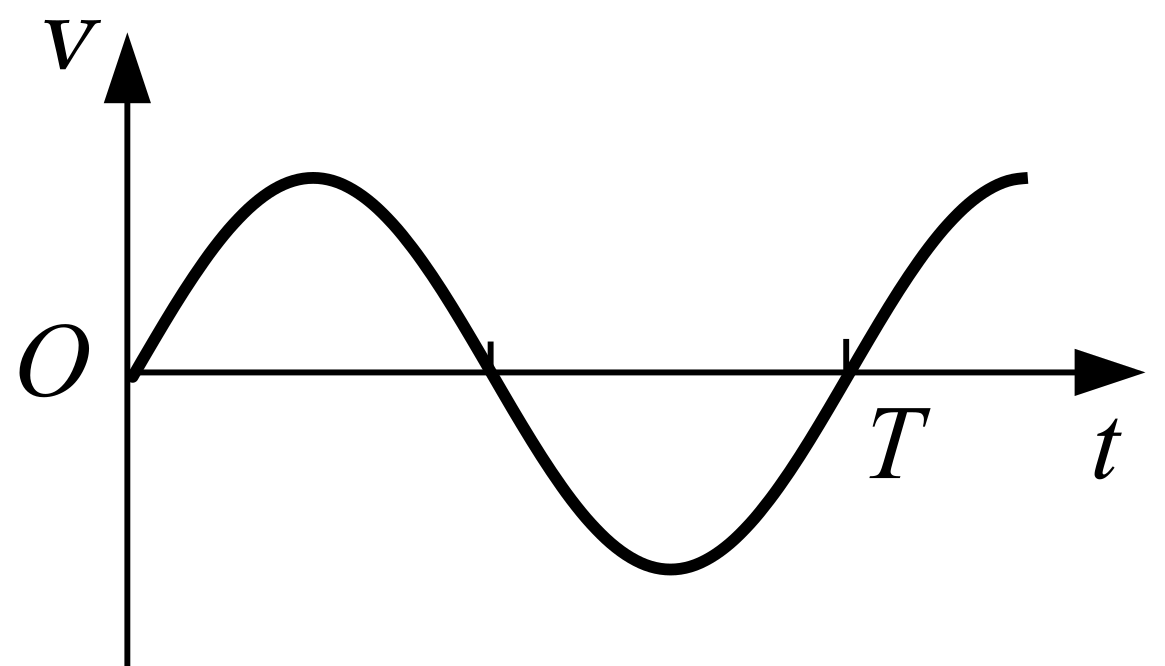
\includegraphics{figs/07a.png}}
{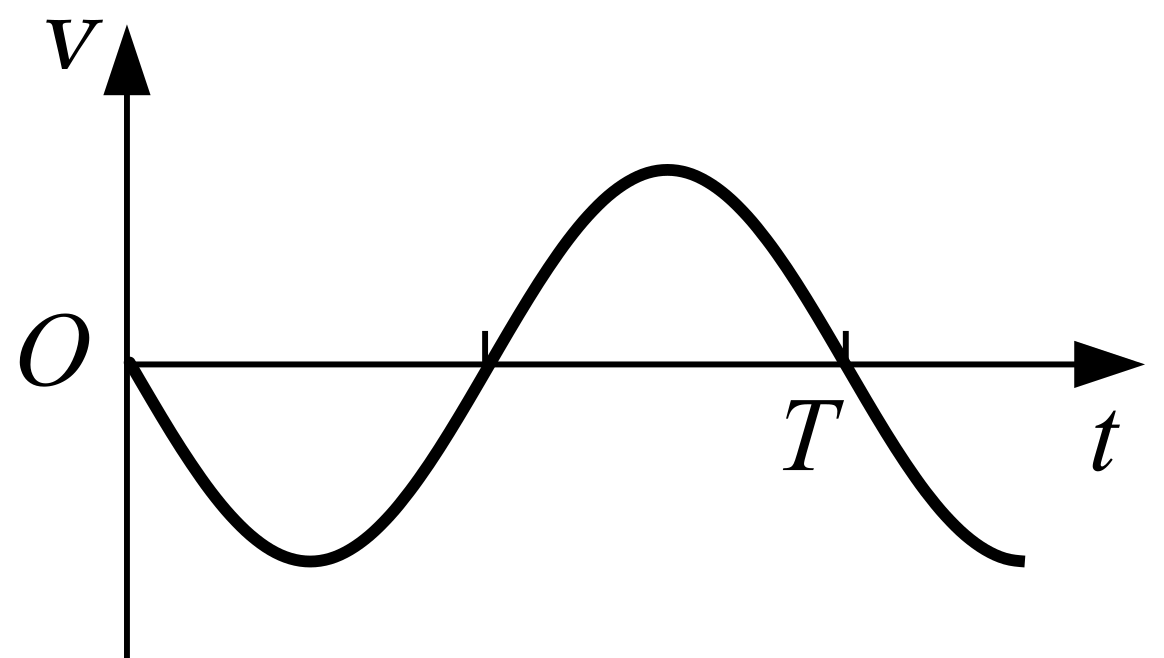
\includegraphics{figs/07b.png}}
{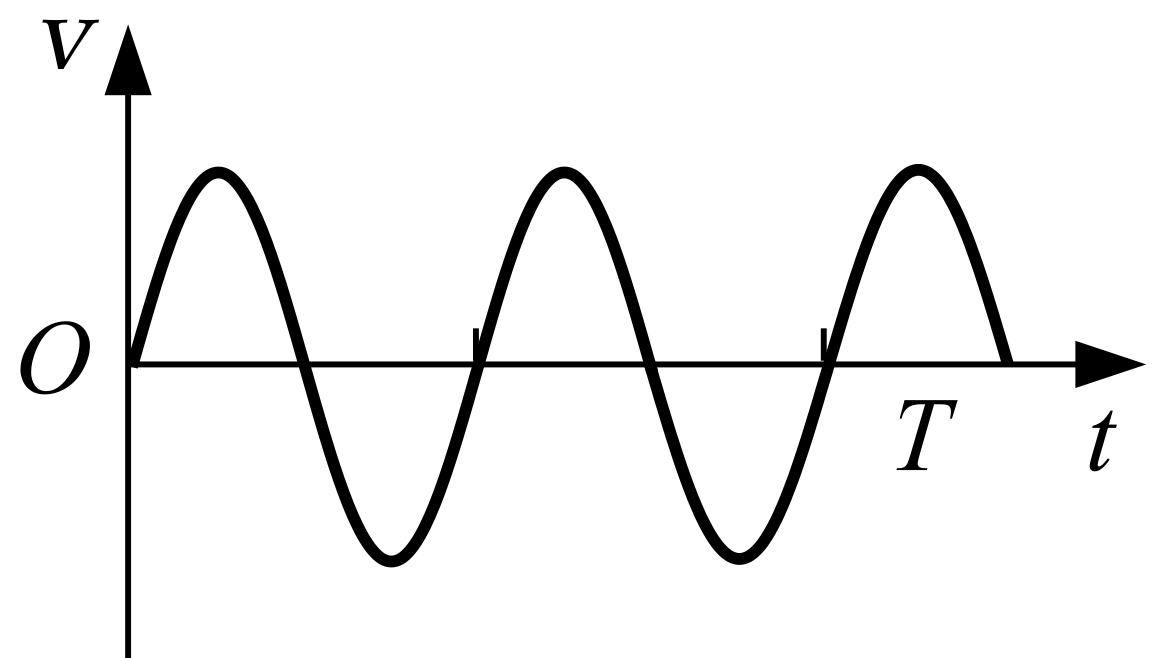
\includegraphics{figs/07c.png}}
{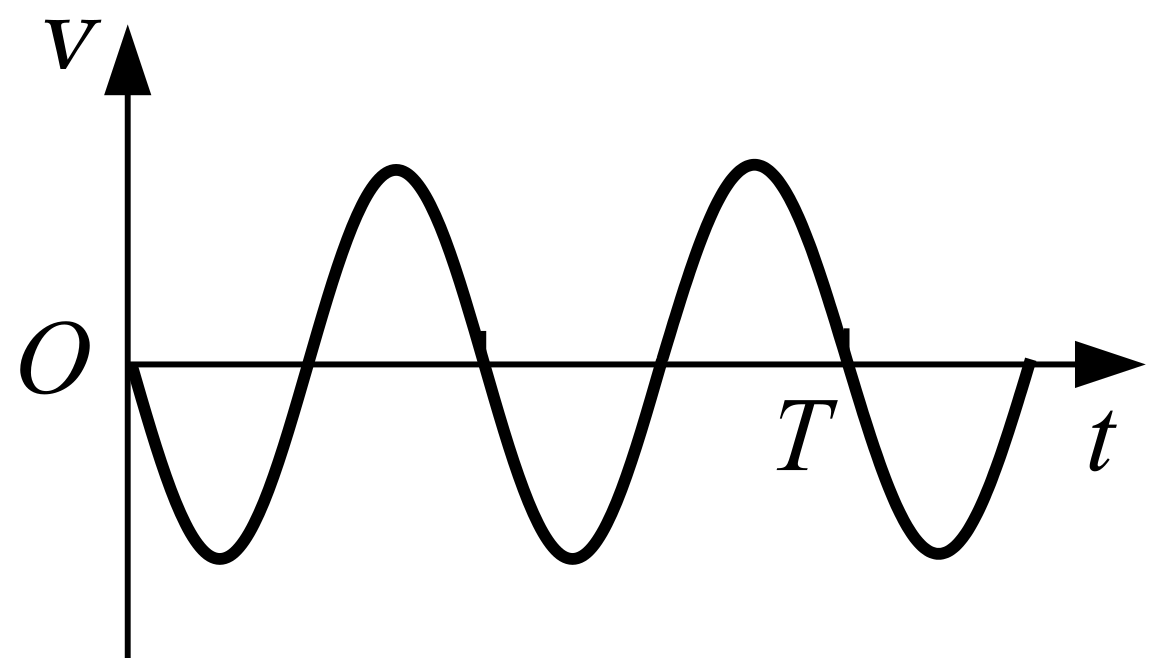
\includegraphics{figs/07d.png}}
%% answer: B
%% memo:
\memoanswer{
由振动图象可得，在 $t=0$ 时刻质点的速度为零，之后向负方向运动，速度先负向增大后负向减小，且振动周期为 $T$，故 B 正确。
}

\item
%% number: 8
%% paperName: 2014年上海高考第 8 题 2 分
%% typeId: 1
%% type: 单选题
%% chapter: 直线运动
%% point: 竖直上下抛运动
%% method: 无
%% score: 2
%% degree: 909
%% duplicateId: 0
%% body:
在离地高 $h$ 处，沿竖直方向同时向上和向下抛出两个小球，它们的初速度大小均为 $v$，不计空气阻力，两球落地的时间差为\xzanswer{A}
\fourchoices[answer=A]
{$\frac{2v}{g}$}
{$\frac{v}{g}$}
{$\frac{2h}{v}$}
{$\frac{h}{v}$}
%% answer: A
%% memo:
\memoanswer{
两球落地的时间差为竖直上抛的小球从抛出到返回出发点的时间，$t=\frac{-v-v}{-g}=\frac{2v}{g}$，故 A 正确。
}

\item
%% number: 9
%% paperName: 2014年上海高考第 9 题 3 分
%% typeId: 1
%% type: 单选题
%% chapter: 力物体的平衡
%% point: 动态平衡
%% method: 无
%% score: 3
%% degree: 944
%% duplicateId: 0
%% body:
如图，光滑的四分之一圆弧轨道 AB 固定在竖直平面内，A 端与水平面相切，穿在轨道上的小球在拉力 $F$ 作用下，缓慢地由 A 向 B 运动，$F$ 始终沿轨道的切线方向，轨道对球的弹力为 $N$，在运动过程中\xzanswer{A}
\onepicture[h=3.4cm, align=right]{\includesvg{figs/09}}
\fourchoices[answer=A]
{$F$ 增大，$N$ 减小}
{$F$ 减小，$N$ 减小}
{$F$ 增大，$N$ 增大}
{$F$ 减小，$N$ 增大}
%% answer: A
%% memo:
\memoanswer{
设小球与圆心的连线与竖直方向的夹角为 $\theta$，由共点力的平衡条件得 $F = mg\sin\theta$，$F_N = mg\cos\theta$，$\theta$ 逐渐变大，所以 $F$ 变大，$F_N$ 变小，故 A 正确。
}

\item
%% number: 10
%% paperName: 2014年上海高考第 10 题 3 分
%% typeId: 1
%% type: 单选题
%% chapter: 气体性质
%% point: 液柱移动定性分析
%% method: 无
%% score: 3
%% degree: 941
%% duplicateId: 0
%% body:
如图，竖直放置、开口向下的试管内用水银封闭一段气体，若试管自由下落，管内气体\xzanswer{B}
\onepicture[h=4.0cm, align=right]{\includesvg{figs/10}}
\fourchoices[answer=B]
{压强增大，体积增大}
{压强增大，体积减小}
{压强减小，体积增大}
{压强减小，体积减小}
%% answer: B
%% memo:
\memoanswer{
试管自由下落处于完全失重状态，一切与重力有关的现象都消失了，管内气体的压强由原来的 $p_0 - \rho gh$ 变为大气压强 $p_0$，是增大的，又由 $\frac{pV}{T} = C$ 知，温度不变，故气体的体积变小，故 B 正确。
}

\item
%% number: 11
%% paperName: 2014年上海高考第 11 题 3 分
%% typeId: 1
%% type: 单选题
%% chapter: 功和能
%% point: 机械能守恒定律
%% method: 无
%% score: 3
%% degree: 786
%% duplicateId: 0
%% body:
静止在地面上的物体在竖直向上的恒力作用下上升，在某一高度撤去恒力。不计空气阻力，在整个上升过程中，物体机械能随时间变化关系是\xzanswer{C}
\fourchoices[answer=C, ispicture=true, h=2.0cm]
{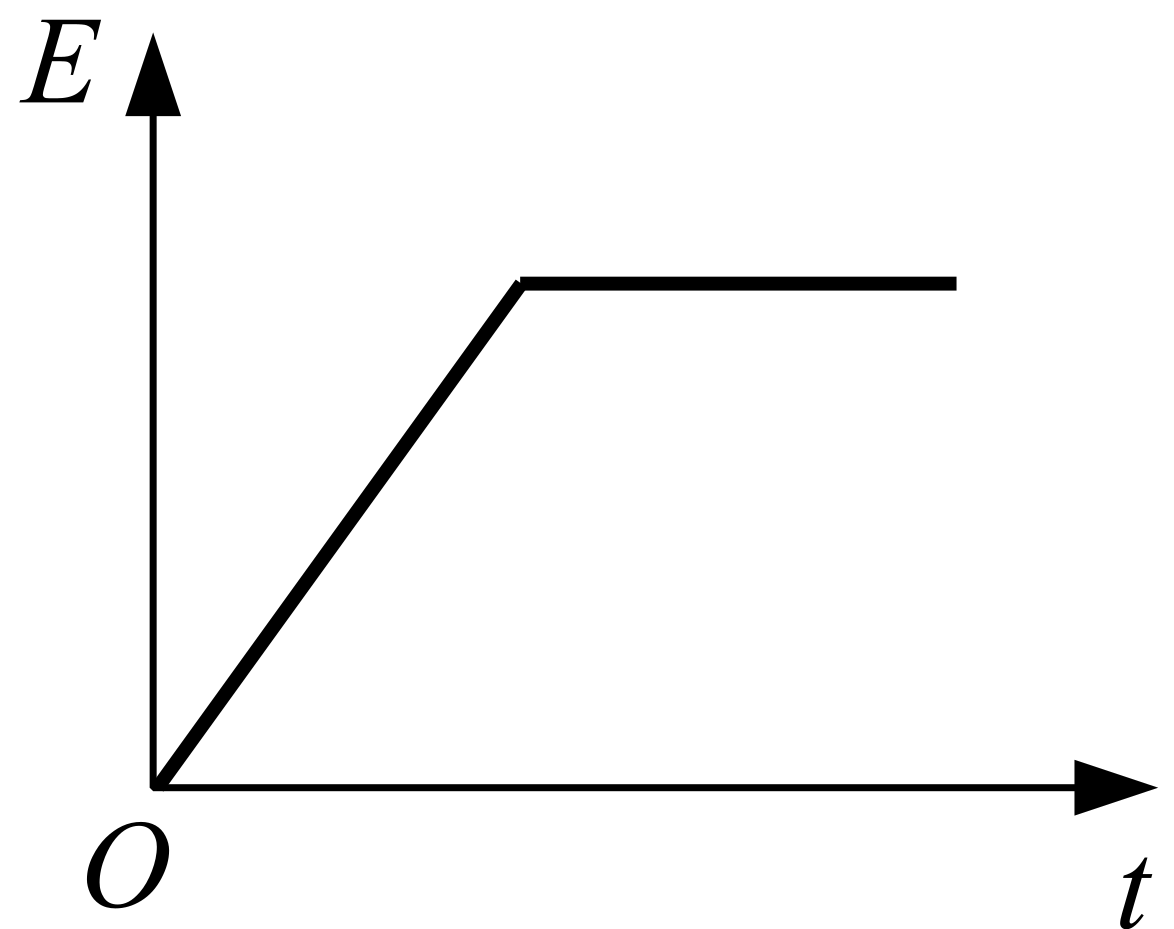
\includegraphics{figs/11a.png}}
{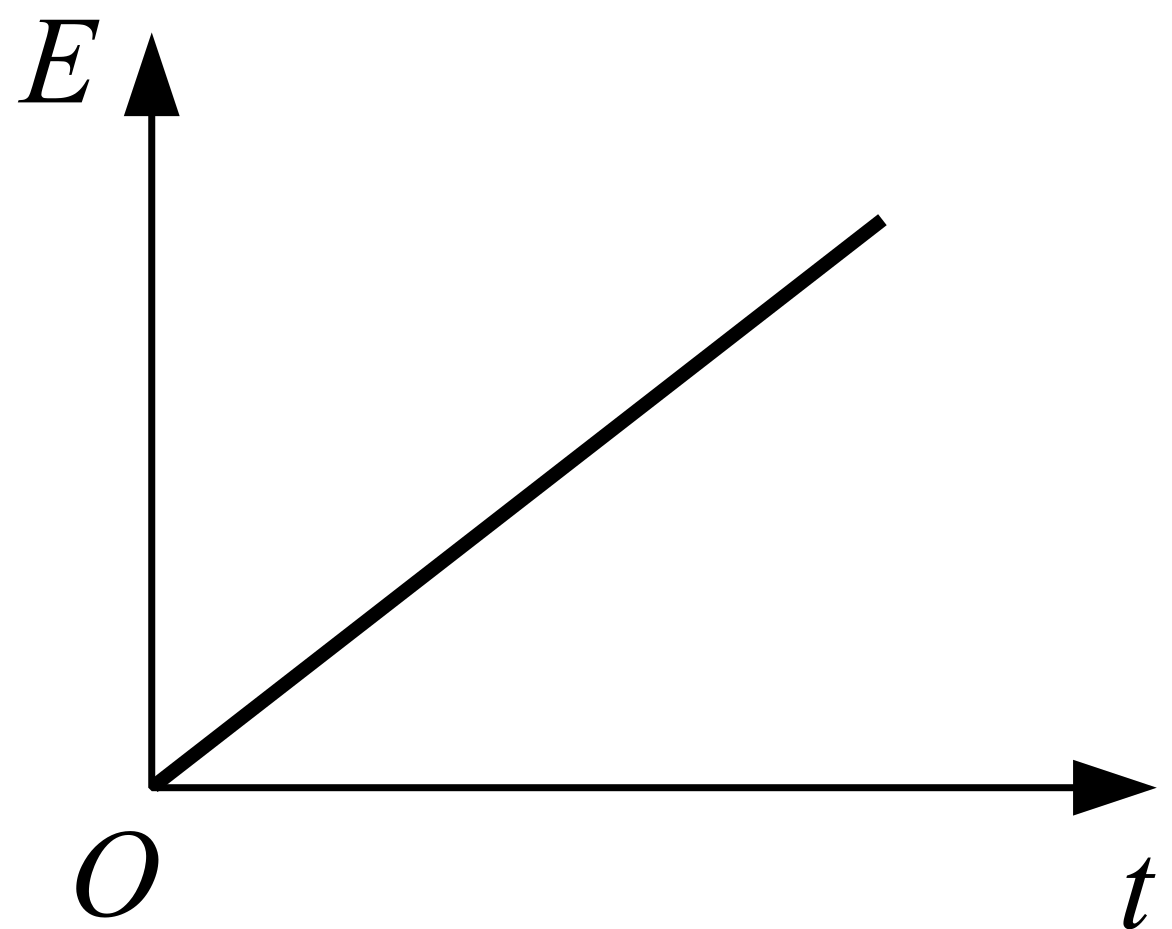
\includegraphics{figs/11b.png}}
{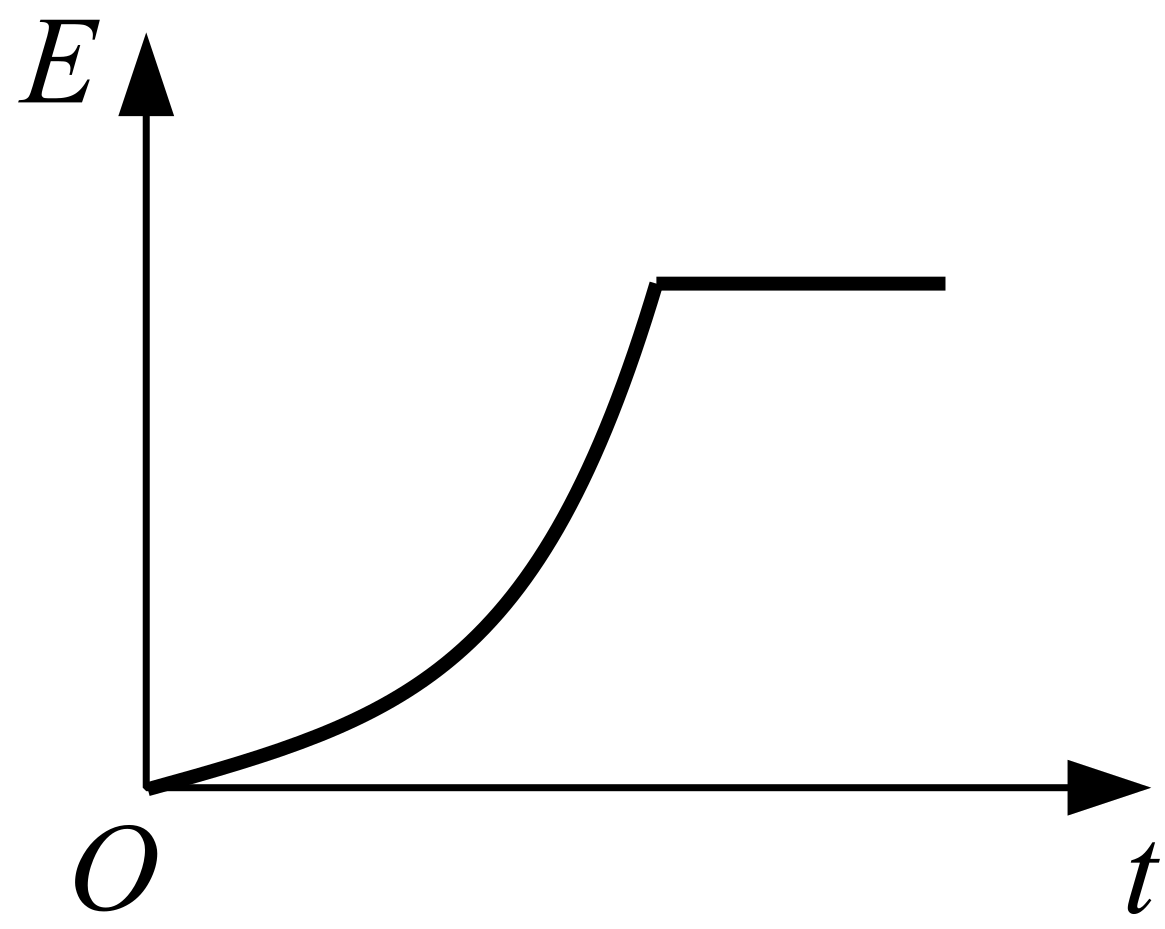
\includegraphics{figs/11c.png}}
{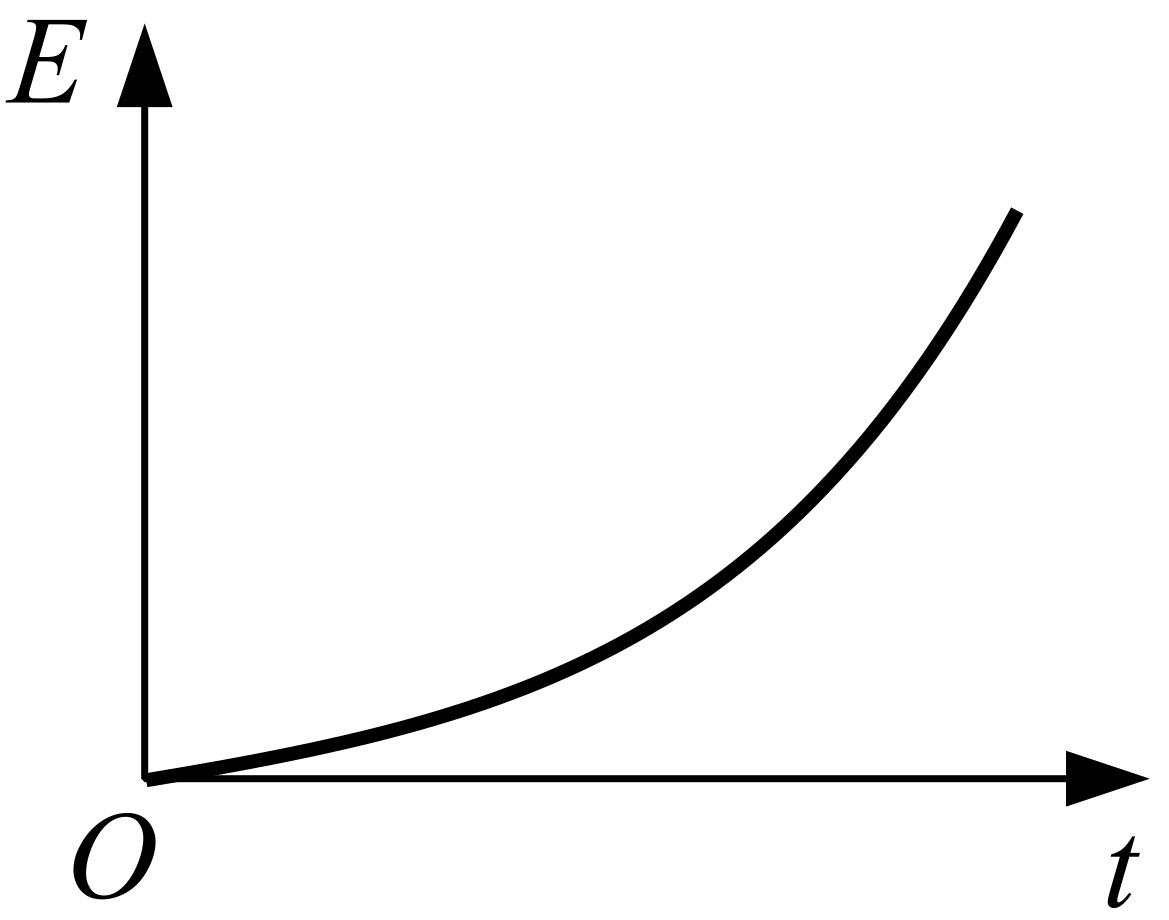
\includegraphics{figs/11d.png}}
%% answer: C
%% memo:
\memoanswer{
物体在恒力作用下的上升过程中，恒力做正功，物体的机械能变大，$E = Fx = F \times \frac{1}{2}at^2$，又因 $a$ 恒定，图线为开口向上的抛物线，撤掉恒力后，只有重力做功，机械能守恒，图线是水平的直线，故 C 正确。
}

\item
%% number: 12
%% paperName: 2014年上海高考第 12 题 3 分
%% typeId: 1
%% type: 单选题
%% chapter: 磁场
%% point: 磁力矩
%% method: 无
%% score: 3
%% degree: 734
%% duplicateId: 0
%% body:
如图，在磁感应强度为 $B$ 的匀强磁场中，面积为 $S$ 的矩形刚性导线框 abcd 可绕过 ad 边的固定轴 OO$'$ 转动，磁场方向与线框平面垂直，在线框中通以电流强度为 $I$ 的稳恒电流，并使线框与竖直平面成 $\theta$ 角，此时 bc 边受到相对 OO$'$ 轴的安培力力矩大小为\xzanswer{A}
\onepicture[h=3.4cm, align=right]{\includesvg{figs/12}}
\fourchoices[answer=A]
{$BIS\sin\theta$}
{$BIS\cos\theta$}
{$BIS/\sin\theta$}
{$BIS/\cos\theta$}
%% answer: A
%% memo:
\memoanswer{
由题意知，安培力大小为 $F = BI \cdot bc$，安培力的力矩 $F \cdot ab\sin\theta = BIS\sin\theta$，故 A 正确。
}

\item
%% number: 13
%% paperName: 2014年上海高考第 13 题 3 分
%% typeId: 1
%% type: 单选题
%% chapter: 曲线运动
%% point: 圆周运动的应用
%% method: 无
%% score: 3
%% degree: 872
%% duplicateId: 0
%% body:
如图，带有一白点的黑色圆盘，可绕过其中心、垂直于盘面的轴匀速转动，每秒沿顺时针方向旋转 30 圈，在暗室中用每秒闪光 31 次的频闪光源照射圆盘，观察到白点每秒沿\xzanswer{D}
\onepicture[h=3.2cm, align=right]{\includesvg{figs/13}}
\fourchoices[answer=D]
{顺时针旋转 31 圈}
{逆时针旋转 31 圈}
{顺时针旋转 1 圈}
{逆时针旋转 1 圈}
%% answer: D
%% memo:
\memoanswer{
圆盘的转动频率小于闪光的频率，我们看着白点好像是逆时针转动，且每秒转一圈，故 D 正确。
}

\item
%% number: 14
%% paperName: 2014年上海高考第 14 题 3 分
%% typeId: 1
%% type: 单选题
%% chapter: 机械波
%% point: 波的图象
%% method: 无
%% score: 3
%% degree: 699
%% duplicateId: 0
%% body:
一列横波沿水平放置的弹性绳向右传播，绳上两质点 A、B 的平衡位置相距 3/4 波长，B 位于 A 右方，$t$ 时刻 A 位于平衡位置上方且向上运动，再经过 1/4 周期，B 位于平衡位置\xzanswer{D}
\fourchoices[answer=D]
{上方且向上运动}
{上方且向下运动}
{下方且向上运动}
{下方且向下运动}
%% answer: D
%% memo:
\memoanswer{
$t$ 时刻 A 位于平衡位置上方且向上运动，且 A、B 相距 $\frac{3}{4}$ 波长，则 $t$ 时刻 B 位于平衡位置上方，且向下运动，再过 $\frac{1}{4}$ 个周期 B 的振动情况与 $t$ 时刻 A 的振动情况相反，即位于平衡位置下方且向下运动，故 D 正确。
}

\item
%% number: 15
%% paperName: 2014年上海高考第 15 题 3 分
%% typeId: 1
%% type: 单选题
%% chapter: 电路
%% point: 输出功率极值
%% method: 极值
%% score: 3
%% degree: 450
%% duplicateId: 0
%% body:
将阻值随温度升高而减小的热敏电阻 Ⅰ 和 Ⅱ 串联，接在不计内阻的稳压电源两端，开始时 Ⅰ 和 Ⅱ 阻值相等，保持 Ⅰ 温度不变，冷却或加热 Ⅱ，则 Ⅱ 的电功率在\xzanswer{C}
\fourchoices[answer=C]
{加热时变大，冷却时变小}
{加热时变小，冷却时变大}
{加热或冷却都变小}
{加热或冷却都变大}
%% answer: C
%% memo:
\memoanswer{
加热时电阻变小，冷却时电阻变大，将 Ⅰ 等效为电源的内阻，Ⅱ 的电阻等于 Ⅰ 的电阻时，Ⅱ 的功率最大，所以无论加热还是冷却，Ⅱ 的电功率都变小，故 C 正确。
}

\item
%% number: 16
%% paperName: 2014年上海高考第 16 题 3 分
%% typeId: 1
%% type: 单选题
%% chapter: 功和能
%% point: 动能定理
%% method: 图象法
%% score: 3
%% degree: 687
%% duplicateId: 0
%% body:
如图，竖直平面内的轨道 Ⅰ 和 Ⅱ 都由两段细直杆连接而成，两轨道长度相等，用相同的水平恒力将穿在轨道最低点 B 的静止小球，分别沿 Ⅰ 和 Ⅱ 推至最高点 A，所需时间分别为 $t_{1}$、$t_{2}$，动能增量分别为 $\Delta E_{k1}$、$\Delta E_{k2}$，假定球在经过轨道转折点前后速度大小不变，且球与 Ⅰ 和 Ⅱ 轨道间的动摩擦因数相等，则\xzanswer{B}
\onepicture[w=6.0cm, align=right]{\includesvg{figs/16}}
\fourchoices[answer=B]
{$\Delta E_{k1} > \Delta E_{k2}$，$t_{1} > t_{2}$}
{$\Delta E_{k1} = \Delta E_{k2}$，$t_{1} > t_{2}$}
{$\Delta E_{k1} > \Delta E_{k2}$，$t_{1} < t_{2}$}
{$\Delta E_{k1} = \Delta E_{k2}$，$t_{1} < t_{2}$}
%% answer: B
%% memo:
\memoanswer{
两种情况下，水平恒力和摩擦力对球做的总功相等，所以 $\Delta E_{k1} = \Delta E_{k2}$，但由于第 Ⅱ 种情况的平均速度大，所以用的时间就少，$t_1 > t_2$，故 B 正确。
}

\item
%% number: 17
%% paperName: 2014年上海高考第 17 题 4 分
%% typeId: 2
%% type: 多选题
%% chapter: 电磁感应
%% point: 楞次定律推广
%% method: 无
%% score: 4
%% degree: 849
%% duplicateId: 0
%% body:
如图，匀强磁场垂直于软导线回路平面，由于磁场发生变化，回路变为圆形，则该磁场\xzanswer{CD}
\onepicture[h=2.8cm, align=right]{\includesvg{figs/17}}
\fourchoices[answer=CD]
{逐渐增强，方向向外}
{逐渐增强，方向向里}
{逐渐减弱，方向向外}
{逐渐减弱，方向向里}
%% answer: CD
%% memo:
\memoanswer{
圆形的面积比题图所示的面积大，由楞次定律“增缩减扩”的结论，该磁场可能是方向向里减弱，也可能是方向向外减弱，故 CD 正确。
}

\item
%% number: 18
%% paperName: 2014年上海高考第 18 题 4 分
%% typeId: 2
%% type: 多选题
%% chapter: 电路
%% point: 动态分析
%% method: 无
%% score: 4
%% degree: 631
%% duplicateId: 0
%% body:
如图，电路中定值电阻阻值 $R$ 大于电源内阻阻值 $r$，将滑动变阻器滑片向下滑动，理想电压表 V$_{1}$、V$_{2}$、V$_{3}$ 示数变化量的绝对值分别为 $\Delta U_{1}$、$\Delta U_{2}$、$\Delta U_{3}$，理想电流表 A 示数变化量的绝对值为 $\Delta I$，则\xzanswer{ACD}
\onepicture[w=6.5cm, align=right]{\includesvg{figs/18}}
\fourchoices[answer=ACD]
{A 的示数增大}
{V$_{2}$ 的示数增大}
{$\Delta U_{3}$ 与 $\Delta I$ 的比值大于 $r$}
{$\Delta U_{1}$ 大于 $\Delta U_{2}$}
%% answer: ACD
%% memo:
\memoanswer{
定值电阻 $R$ 与滑动变阻器串联，滑动变阻器的滑片向下移动，滑动变阻器接入电路的电阻变小，A 的示数增大，故 A 正确；V$_{2}$ 的示数是路端电压，根据 $U_2 = E - Ir$ 可知，V$_{2}$ 的示数变小，故 B 错误；又 $E = U_3 + I(R + r)$，则 $\Delta U_3$ 和 $\Delta I$ 的比值等于 $R + r$，大于 $r$，故 C 正确；$\Delta U_1$ 是 $R$ 两端电压的变化量，$\Delta U_2$ 是路端电压变化量，$\Delta U_1$ 大于 $\Delta U_2$，故 D 正确。

首先应将此电路化简成一个易于识别的电路如右图所示。电流表 A 测的是干路电流，电压表 V$_{1}$ 测的是定值电阻 $R$ 两端的电压，电压表 V$_{2}$ 测的是电源两端的电压，电压表 V$_{3}$ 测的是滑动变阻器两端的电压。

\onepicture[w=5.6cm, align=right]{figs/18_an.png}

当滑动变阻器滑片向下滑动时，接入电路的有效电阻减小，整个电路的电流 $I$ 变大，则 A 表和 V$_{1}$ 表的示数变大，选项（A）正确。

由 $U_{2}=E-Ir$，$E$、$r$ 不变，$I$ 增大，所以 $U_{2}$ 减小，选项（B）错误。

由 $\frac{\Delta U_{3}}{\Delta I} = R + r$ 可知，$\frac{\Delta U_{3}}{\Delta I} > r$，选项（C）正确。

由 $\frac{\Delta U_{1}}{\Delta I} = R$、$\frac{\Delta U_{2}}{\Delta I} = r$，且题中已知 $R > r$，可得 $\Delta U_{1} > \Delta U_{2}$，选项（D）正确。
}

\item
%% number: 19
%% paperName: 2014年上海高考第 19 题 4 分
%% typeId: 2
%% type: 多选题
%% chapter: 电场
%% point: 电场中的图象
%% method: 无
%% score: 4
%% degree: 673
%% duplicateId: 0
%% body:
静电场在 $x$ 轴上的场强 $E$ 随 $x$ 的变化关系如图所示，$x$ 轴正方向为场强正方向，带正电的点电荷沿 $x$ 轴运动，则点电荷\xzanswer{BC}
\onepicture[w=7.0cm, align=right]{\includesvg{figs/19}}
\fourchoices[answer=BC]
{在 $x_{2}$ 和 $x_{4}$ 处电势能相等}
{由 $x_{1}$ 运动到 $x_{3}$ 的过程中电势能增大}
{由 $x_{1}$ 运动到 $x_{4}$ 的过程中电场力先增大后减小}
{由 $x_{1}$ 运动到 $x_{4}$ 的过程中电场力先减小后增大}
%% answer: BC
%% memo:
\memoanswer{
正点电荷从 $x_{2}$ 移动到 $x_{4}$，电场力做负功，所以点电荷在 $x_{2}$ 和 $x_{4}$ 处的电势能不相等，故 A 错误；由 $x_{1}$ 运动到 $x_{3}$ 过程中，电场力做负功，电势能增大，故 B 正确；由 $x_{1}$ 运动到 $x_{4}$ 过程中，场强先变大后变小，电场力也先增大后减小，故 C 正确 D 错误。
}

\item
%% number: 20
%% paperName: 2014年上海高考第 20 题 4 分
%% typeId: 2
%% type: 多选题
%% chapter: 气体性质
%% point: 液柱移动定性分析
%% method: 无
%% score: 4
%% degree: 457
%% duplicateId: 0
%% body:
如图，在水平放置的刚性气缸内用活塞封闭两部分气体 A 和 B，质量一定的两活塞用杆连接，气缸内两活塞间保持真空，活塞与气缸壁之间无摩擦，左侧活塞面积较大，A、B 的初始温度相同，略抬高气缸左端使之倾斜，再使升高相同温度，气体最终达到稳定状态。若始末状态 A、B 的压强变化量 $\Delta p_{A}$、$\Delta p_{B}$ 均大于零，对活塞压力的变化量为 $\Delta F_{A}$、$\Delta F_{B}$，则\xzanswer{AD}
\onepicture[w=6.8cm, align=right]{\includesvg{figs/20}}
\fourchoices[answer=AD]
{A 体积增大}
{A 体积减小}
{$\Delta F_{A} > \Delta F_{B}$}
{$\Delta p_{A} < \Delta p_{B}$}
%% answer: AD
%% memo:
\memoanswer{
升高相同的温度，活塞要向右移动一定距离，A 体积增大，故 A 正确 B 错误；两活塞用同一轻杆相连，所以 $(p_{A}+\Delta p_{A})S_{A}=(p_{B}+\Delta p_{B})S_{B}$，又初始时 $p_{A}S_{A}=p_{B}S_{B}$，所以 $\Delta p_{A}<\Delta p_{B}$，故 C 错误 D 正确。
}

\item
%% number: 21
%% paperName: 2014年上海高考第 21 题 4 分
%% typeId: 3
%% type: 填空题
%% chapter: 运动和力
%% point: 牛顿第一定律
%% method: 无
%% score: 4
%% degree: 795
%% duplicateId: 0
%% body:
牛顿第一定律表明，力是物体\tkanswer[2.2cm]{运动状态}发生变化的原因；该定律引出的一个重要概念是\tkanswer[1.6cm]{惯性}。
%% answer: 运动状态，惯性
%% memo:
\memoanswer{
牛顿第一定律说明，力是改变物体运动状态（速度）的原因，任何物体在任何状态下都具有惯性。
}

\item
%% number: 22
%% paperName: 2014年上海高考第 22 题 4 分
%% typeId: 3
%% type: 填空题
%% chapter: 曲线运动
%% point: 人造地球卫星
%% method: 无
%% score: 4
%% degree: 792
%% duplicateId: 0
%% body:
本题为分叉题，分 A、B 两类，考生可任选一类答题，若两类试题均做，一律按 A 类题计分。

\textbf{A．}动能相等的两物体 A、B 在光滑水平面上沿同一直线相向而行，它们的速度大小之比 $v_{A}:v_{B} = 2:1$，则动量大小之比 $p_{A}:p_{B} =$\tkanswer[1.2cm]{$1:2$}，两者碰后粘在一起运动，其总动量与 A 原来动量大小之比 $p:p_{A}=$\tkanswer[1.2cm]{$1:1$}。

\textbf{B．}动能相等的两颗人造地球卫星 A、B 的轨道半径之比为 $R_{A}:R_{B} = 1:2$，它们的角速度之比 $\omega_{A}:\omega_{B} =$\tkanswer[2.2cm]{$2\sqrt 2:1$}，质量之比 $m_{A}:m_{B}=$\tkanswer[1.2cm]{$1:2$}。
%% answer: A．1:2，1:1；B．$2\sqrt 2:1$，1:2
%% memo:
\memoanswer{
\textbf{A．}由动能定义可知 $E_{kA}=\frac{1}{2}m_{A}v_{A}^{2}$、$E_{kB}=\frac{1}{2}m_{B}v_{B}^{2}$，且 $E_{kA}=E_{kB}$，由动量定义可知 $p_{A}=m_{A}v_{A}$、$p_{B}=m_{B}v_{B}$，代入速度比解得 $\frac{p_{A}}{p_{B}}=\frac{1}{2}$；由动量守恒定律可知，两者碰撞粘合后的总动量与 A 原来的动量之比为 $\frac{|p_{A}-p_{B}|}{p_{A}}=\frac{1}{1}$。

\textbf{B．}由动能定义、线速度与角速度关系可知 $E_{\mathrm{kA}} = \frac{1}{2} m_A (R_A \omega_A)^2$、$E_{\mathrm{kB}} = \frac{1}{2} m_B (R_B \omega_B)^2$，且 $E_{\mathrm{kA}} = E_{\mathrm{kB}}$，对两卫星的环绕运动，由牛顿第二定律及万有引力定律得 $G \frac{M m_A}{R_A^2} = m_A R_A \omega_A^2$、$G \frac{M m_B}{R_B^2} = m_B R_B \omega_B^2$，代入轨道半径比解得 $\frac{\omega_A}{\omega_B} = \frac{2\sqrt{2}}{1}$，$\frac{m_A}{m_B} = \frac{1}{2}$。
}

\item
%% number: 23
%% paperName: 2014年上海高考第 23 题 4 分
%% typeId: 3
%% type: 填空题
%% chapter: 直线运动
%% point: 多段匀变速直线运动
%% method: 无
%% score: 4
%% degree: 771
%% duplicateId: 0
%% body:
如图，两光滑斜面在 B 处连接，小球由 A 处静止释放，经过 B、C 两点时速度大小分别为 $3\Ums$ 和 $4\Ums$，AB $=$ BC。设球经过 B 点前后速度大小不变，则球在 AB、BC 段的加速度大小之比为\tkanswer[1.6cm]{$9:7$}，球由 A 运动到 C 的过程中平均速率为\tkanswer[1.6cm]{2.1}$\Ums$。
\onepicture[w=6.0cm, align=right]{\includesvg{figs/23}}
%% answer: 9:7，2.1
%% memo:
\memoanswer{
设 $AB = BC = s$，对小球在 A、B 间和 B、C 间的运动，由匀变速直线运动规律得 $v_{B}^{2} = 2a_{1}s$ 和 $v_{C}^{2} - v_{B}^{2} = 2a_{2}s$，解得 $\frac{a_{1}}{a_{2}} = \frac{9}{7}$；由 $s = \frac{v_{B}}{2}t_{1}$、$s = \frac{v_{B} + v_{C}}{2}t_{2}$、$\overline{v} = \frac{2s}{t_{1} + t_{2}}$，解得 $\overline{v} = 2.1\Ums$。
}

\item
%% number: 24
%% paperName: 2014年上海高考第 24 题 4 分
%% typeId: 3
%% type: 填空题
%% chapter: 曲线运动
%% point: 平抛运动
%% method: 无
%% score: 4
%% degree: 608
%% duplicateId: 0
%% body:
如图，宽为 $L$ 的竖直障碍物上开有间距 $d = 0.6\Um$ 的矩形孔，其下沿离地高 $h = 1.2\Um$，离地高 $H = 2\Um$ 的质点与障碍物相距 $x$。在障碍物以 $v_{0} = 4\Ums$ 匀速向左运动的同时，质点自由下落，为使质点能穿过该孔，$L$ 的最大值为\tkanswer[1.2cm]{0.8}$\Um$；若 $L = 0.6\Um$，$x$ 的取值范围是\tkanswer[3.8cm]{$0.8\Um \le x \le 1\Um$}。（取 $g = 10\Umsq$）
\onepicture[h=4.6cm, align=right]{\includesvg{figs/24}}
%% answer: 0.8，$0.8\Um \le x \le 1\Um$
%% memo:
\memoanswer{
对小球的自由落体运动有 $H - h - d = \frac{1}{2}gt_{1}^{2}$、$H - h = \frac{1}{2}gt_{2}^{2}$，解得 $t_{2} - t_{1} = 0.2\Us$，则 $L = v_{0}(t_{2} - t_{1}) = 0.8\Um$；若 $L = 0.6\Um$，则 $t_{2} - t_{1}' = \frac{L}{v_{0}} = 0.15\Us$，因此 $x$ 的最小值为 $v_{0}t_{1} = 0.8\Um$，最大值为 $v_{0}(t_{2} - 0.15) = 1.0\Um$。因此，$0.8\Um \le x \le 1.0\Um$。
}

\item
%% number: 25
%% paperName: 2014年上海高考第 25 题 4 分
%% typeId: 3
%% type: 填空题
%% chapter: 电场
%% point: 带电粒子的平衡
%% method: 无
%% score: 4
%% degree: 201
%% duplicateId: 0
%% body:
如图，竖直绝缘墙上固定一带电小球 A，将带电小球 B 用轻质绝缘丝线悬挂在 A 的正上方 C 处，图中 AC $= h$，当 B 静止在与竖直方向夹角 $\theta = 30^{\circ}$ 方向时，A 对 B 的静电力为 B 所受重力的 $\frac{\sqrt 3}{3}$ 倍，则丝线 BC 长度为\tkanswer[2.6cm]{$\frac{\sqrt 3}{3}h$ 或 $\frac{2\sqrt 3}{3}h$}。若 A 对 B 的静电力为 B 所受重力的 0.5 倍，改变丝线长度，使仍能在 $\theta = 30^{\circ}$ 处平衡，以后由于 A 漏电，B 在竖直平面内缓慢运动，到 $\theta = 0^{\circ}$ 处 A 的电荷尚未漏完，在整个漏电过程中，丝线上拉力大小的变化情况是\tkanswer[2.4cm]{先不变后增大}。
\onepicture[h=4.6cm, align=right]{\includesvg{figs/25}}
%% answer: $\frac{\sqrt 3}{3}h$ 或 $\frac{2\sqrt 3}{3}h$；先不变后增大
%% memo:
\memoanswer{
由共点力平衡条件可知，由表示带电小球 B 所受重力、静电力及丝线拉力三力的线段组成的三角形与三角形 ABC 相似，因此 $\frac{h}{G}=\frac{AB}{\frac{\sqrt 3 G}{3}}$，解得 $AB=\frac{\sqrt 3}{3}h$，在三角形 ABC 中，由余弦定理可解得 $BC=\frac{\sqrt 3}{3}h$ 或 $BC=\frac{2\sqrt 3}{3}h$。A 对 B 的静电力恰好是 B 所受重力的 0.5，有 $\frac{h}{G}=\frac{BC}{F_{\mathrm{T}}}$，若 $BC=\frac{\sqrt 3}{3}h$，得 $F_{\mathrm{T}}=\frac{\sqrt 3}{3}G$，若 $BC=\frac{2\sqrt 3}{3}h$，得 $F_{\mathrm{T}}=\frac{2\sqrt 3}{3}G$，可知，A 球漏电过程中，丝线拉力先是大小保持不变，当 $\theta=0^{\circ}$ 时突变（增大）为 $mg$。
}

\item
%% number: 26
%% paperName: 2014年上海高考第 26 题 4 分
%% typeId: 4
%% type: 实验题
%% chapter: 光学
%% point: 光的衍射
%% method: 无
%% score: 4
%% degree: 503
%% duplicateId: 0
%% body:
如图，在“观察光的衍射现象”实验中，保持缝到光屏的距离不变，增加缝宽，屏上衍射条纹间距将\tkanswer[1.2cm]{减小}（选填：“增大”、“减小”或“不变”）；该现象表明，光沿直线传播只是一种近似规律，只有在\tkanswer[3.8cm]{光的波长比障碍物小得多}情况下，光才可以看作是沿直线传播的。
\onepicture[h=3.4cm, align=right]{\includesvg{figs/26}}
%% answer: 减小，光的波长比障碍物小得多
%% memo:
\memoanswer{
由缝宽与衍射图像条纹宽度关系可知，增大缝宽后，衍射条纹宽度减小；当光的波长比障碍物小得多的情况下，光不会发生明显衍射现象，才可看成直线传播。
}

\item
%% number: 27
%% paperName: 2014年上海高考第 27 题 5 分
%% typeId: 4
%% type: 实验题
%% chapter: 气体性质
%% point: 验证玻意耳定律
%% method: 无
%% score: 5
%% degree: 883
%% duplicateId: 0
%% body:
在“用 DIS 研究在温度不变时，一定质量的气体压强与体积的关系”实验中，某同学将注射器活塞置于刻度为 $10\UmL$ 处，然后将注射器连接压强传感器并开始实验，气体体积 $V$ 每增加 $1\UmL$ 测一次压强 $p$，最后得到 $p$ 和 $V$ 的乘积逐渐增大。
\begin{enumerate}
	\item
	由此可推断，该同学的实验结果可能为图\tkanswer[1.2cm]{a}。
	\item
	（单选题）图线弯曲的可能原因是在实验过程中\tkanswer[1.2cm]{C}

	（A）注射器中有异物 \qquad （B）连接软管中存在气体

	（C）注射器内气体温度升高 \qquad （D）注射器内气体温度降低
\end{enumerate}
\twopicture[h=4.4cm, align=right]
{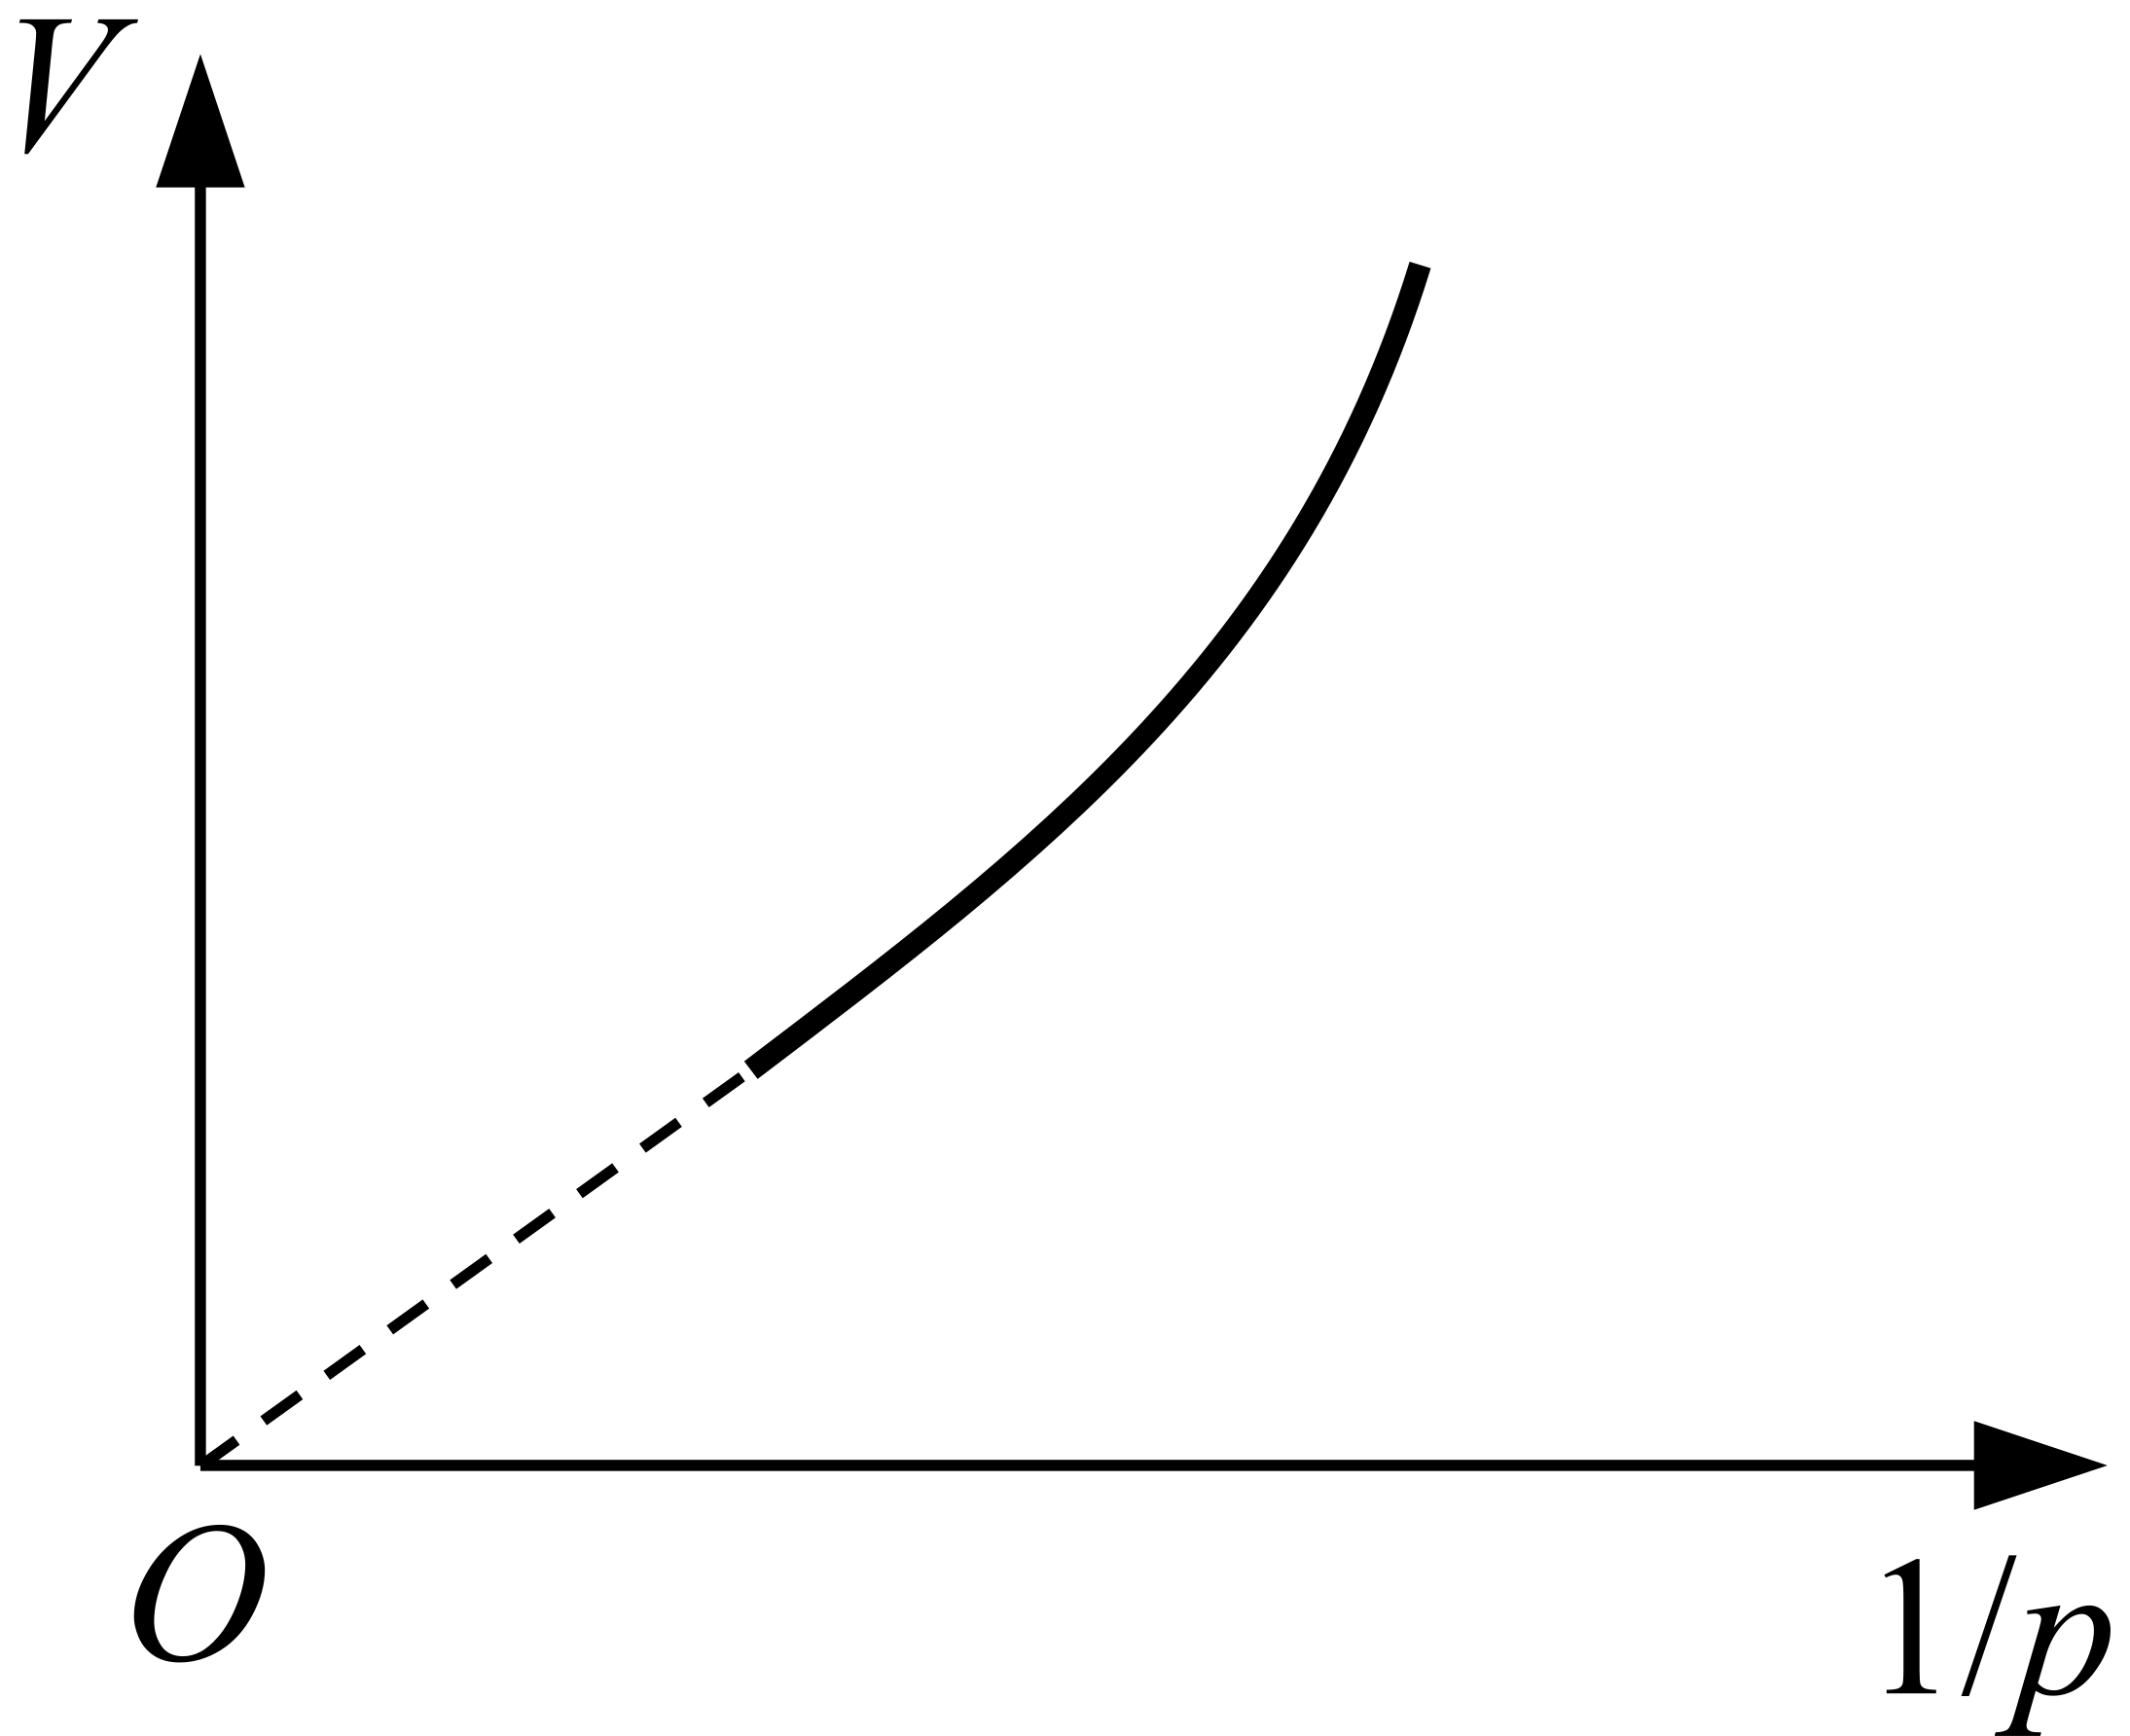
\includegraphics{figs/27a.png}}
{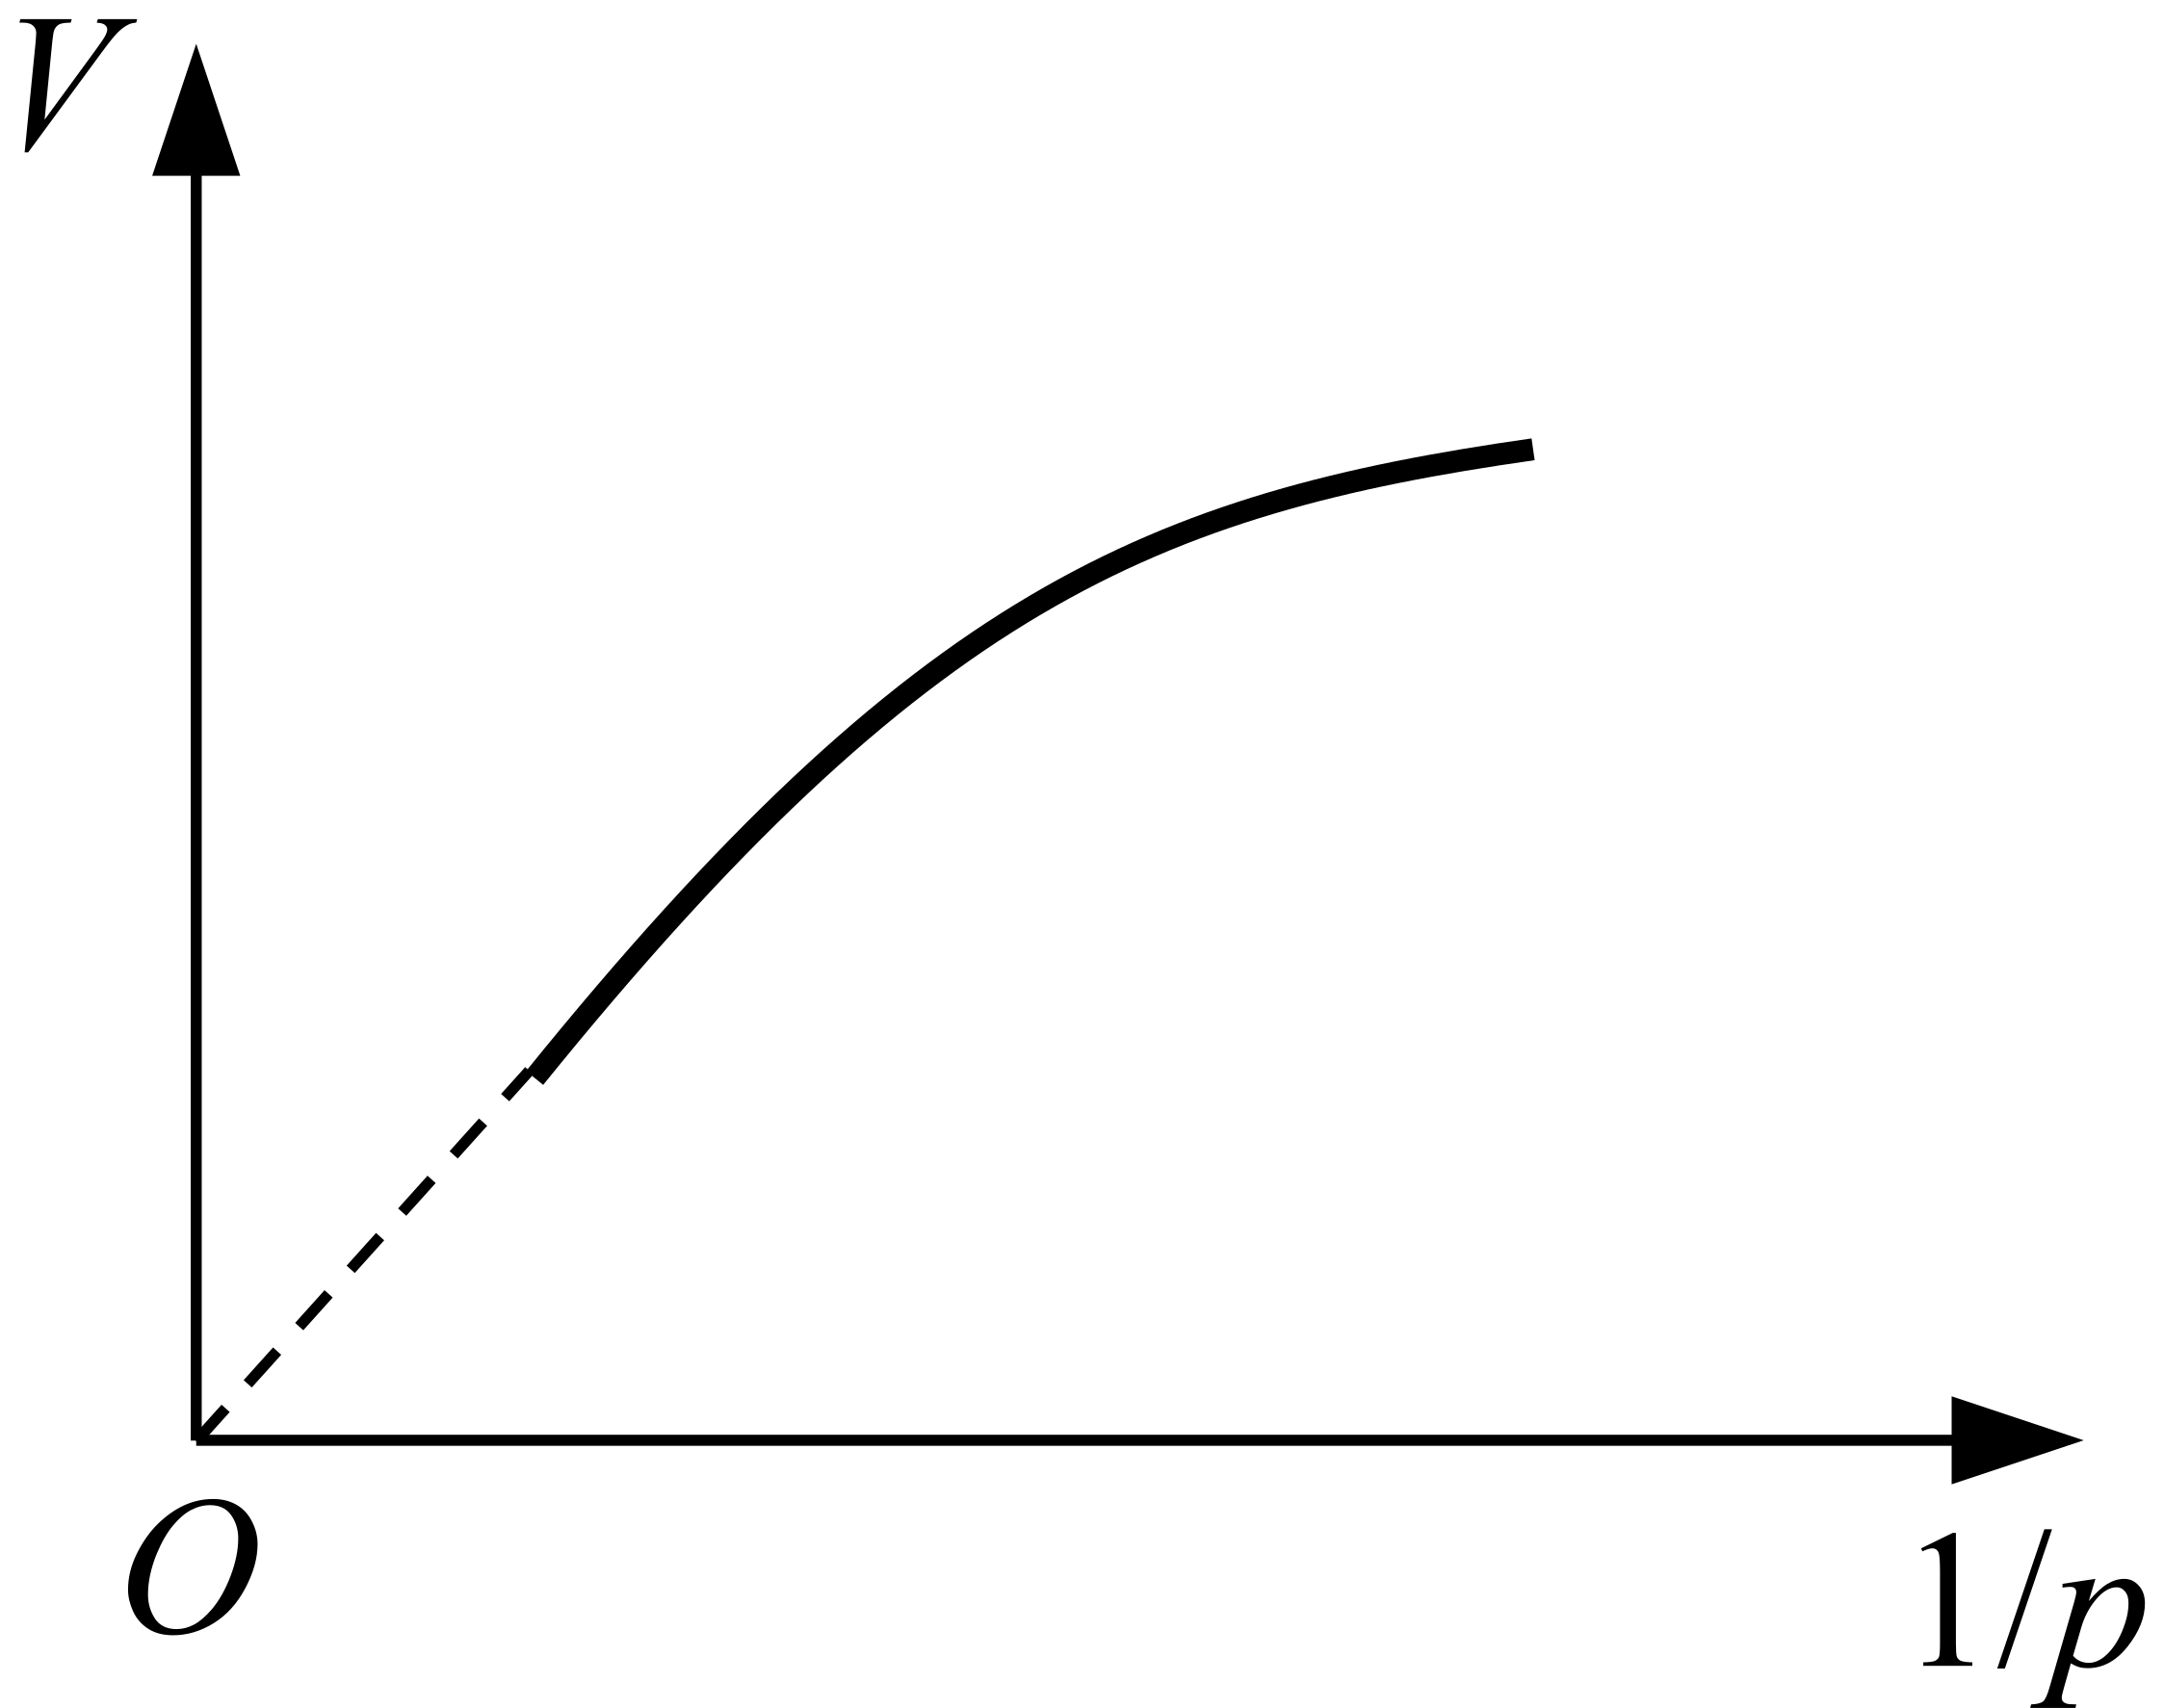
\includegraphics{figs/27b.png}}
%% answer: （1）a（2）C
\jdanswer{
\begin{enumerate}
	\item
	a
	\item
	C
\end{enumerate}
}
%% memo:
\memoanswer{
（1）温度不变时，理想气体的体积与压强成反比，即与压强倒数成正比，因此，实验时得到的图象应是图 a；（2）由理想气体状态方程可知，$V-\frac{1}{p}$ 图象斜率与温度 $T$ 成正比，因此，注射器内气体温度升高，将导致图象发生图 a 所示弯曲，故 ABD 错误 C 正确。
}

\item
%% number: 28
%% paperName: 2014年上海高考第 28 题 7 分
%% typeId: 4
%% type: 实验题
%% chapter: 电路
%% point: 测电动势与内阻
%% method: 无
%% score: 7
%% degree: 450
%% duplicateId: 0
%% body:
在“用 DIS 测电源电动势和内阻”的实验中
\begin{enumerate}
	\item
	将待测电池组、滑动变阻器、电流传感器、电压传感器、定值电阻、电键及若干导线连接成电路如图（a）所示，图中未接导线的 A 端应接在\tkanswer[2.2cm]{C}点（选填：“B”、“C”、“D”或“E”）。
	\item
	实验得到的 $U-I$ 关系如图（b）中的直线 Ⅰ 所示，则电池组的电动势为\tkanswer[1.6cm]{2.8}$\UV$，内电阻阻值为\tkanswer[1.6cm]{2}$\UO$。
	\item
	为了测量定值电阻的阻值，应在图（a）中将“A”重新连接到\tkanswer[2.2cm]{D}点（选填：“B”、“C”、“D”或“E”），所得到的 $U-I$ 关系如图（b）中的直线 Ⅱ 所示，则定值电阻的阻值为\tkanswer[1.6cm]{3}$\UO$。
\end{enumerate}
\twopicture[align=right]
{figs/28a.png}
{\includesvg{figs/28b}}
%% answer: （1）C（2）2.8，2（3）D，3
\jdanswer{
\begin{enumerate}
	\item
	C
	\item
	2.8，2
	\item
	D，3
\end{enumerate}
}
%% memo:
\memoanswer{
（1）图中未接导线 A 所连接的是电压传感器，应将其接在开关的 C 接线柱上。

（2）由图象 Ⅰ 纵截距可知电池组电动势为 $E=2.8\UV$，由图象 Ⅰ 斜率绝对值可知，电池阻内阻为 $r=2.0\UO$。

（3）若将“A”接到“D”点，则图象 Ⅱ 斜率的绝对值表示 $R$ 与电池组内阻之和，因此 $R = 5.0\UO - 2.0\UO = 3.0\UO$。
}

\item
%% number: 29
%% paperName: 2014年上海高考第 29 题 8 分
%% typeId: 4
%% type: 实验题
%% chapter: 机械振动
%% point: 单摆测重力加速度
%% method: 无
%% score: 8
%% degree: 450
%% duplicateId: 0
%% body:
某小组在做“用单摆测定重力加速度”实验后，为进一步探究，将单摆的轻质细线改为刚性重杆。通过查资料得知，这样做成的“复摆”做简谐运动的周期 $T = 2\pi\sqrt{\frac{I_{C} + mr^{2}}{mgr}}$，$I_{C}$ 为由该摆决定的常量，$m$ 为摆的质量，$g$ 为重力加速度，$r$ 为转轴到重心 C 的距离。如图（a）所示，实验时在杆上不同位置打上多个小孔，将其中一个小孔穿在光滑水平轴 O 上，使杆做简谐运动，测量并记录 $r$ 和相应的运动周期 $T$，然后将不同位置的孔穿在轴上重复实验，实验数据见表，并测得摆的质量 $m = 0.50\Ukg$。

\begin{center}
\begin{tabular}{|c|cccccc|}
\hline
$r/\Um$ & 0.45 & 0.40 & 0.35 & 0.30 & 0.25 & 0.20 \\
\hline
$T/\Us$ & 2.11 & 2.14 & 2.20 & 2.30 & 2.43 & 2.64 \\
\hline
\end{tabular}
\end{center}
\begin{enumerate}
	\item
	由实验数据得出图（b）所示拟合直线，图中纵轴表示\tkanswer[2.0cm]{$T^{2}r$}。
	\item
	$I_{C}$ 的国际单位为\tkanswer[2.6cm]{$\Ukg\cdot\Um^{2}$}，由拟合直线得到 $I_{C}$ 的值为\tkanswer[2.6cm]{$0.17\Ukg\cdot\Um^{2}$}（保留到小数点后二位）。
	\item
	若摆的质量测量值偏大，重力加速度 $g$ 的测量值\tkanswer[1.2cm]{不变}。（选填“偏大”、“偏小”或“不变”）
\end{enumerate}
\twopicture[align=right, hA=4.4cm, hB=4.4cm]
{\includesvg{figs/29a}}
{\includesvg{figs/29b}}
%% answer: （1）$T^{2}r$（2）$\Ukg\cdot\Um^{2}$，0.17（3）不变
\jdanswer{
\begin{enumerate}
	\item
	$T^{2}r$
	\item
	$\Ukg\cdot\Um^{2}$，0.17
	\item
	不变
\end{enumerate}
}
%% memo:
\memoanswer{
（1）由 $T=2\pi\sqrt{\frac{I_{C}+mr^{2}}{mgr}}$ 知，$T^{2}r=\frac{4\pi^{2}I_{C}}{mg}+\frac{4\pi^{2}}{g}r^{2}$，因此图象的纵轴表示 $T^{2}r$。

（2）由上式可知，$I_{C}$ 的单位是 $\Ukg\cdot\Um^{2}$；由图象纵截距 $b = 1.25\Us^{2}\cdot\Um$ 及 $b = \frac{4\pi^{2}I_{C}}{mg}$、$m = 0.50\Ukg$、$k = \frac{4\pi^{2}}{g}$ 可得 $I_{C} \approx 0.17\Ukg\cdot\Um^{2}$。

（3）由上式可知图象斜率 $k=\frac{4\pi^{2}}{g}$，则 $g=\frac{4\pi^{2}}{k}$。因此摆的质量的测量值不会影响 $g$ 的测量值。
}

\item
%% number: 30
%% paperName: 2014年上海高考第 30 题 10 分
%% typeId: 6
%% type: 计算题
%% chapter: 气体性质
%% point: 理想气体状态方程
%% method: 无
%% score: 10
%% degree: 650
%% duplicateId: 0
%% body:
如图，一端封闭、粗细均匀的 U 形玻璃管开口向上竖直放置，管内用水银将一段气体封闭在管中，当温度为 $280\UK$ 时，被封闭的气柱长 $L = 22\Ucm$，两边水银面高度差 $h = 16\Ucm$，大气压强 $p_{0} = 76\UcmHg$。
\begin{enumerate}
	\item
	为使左端水银面下降 $3\Ucm$，封闭气体温度应改变为多少？
	\item
	封闭气体的温度重新回到 $280\UK$ 后，为使封闭气体长度变为 $20\Ucm$，需向开口端注入的水银柱长度为多少？
\end{enumerate}
\onepicture[h=4.4cm, align=right]{\includesvg{figs/30}}
%% answer: （1）$T_{2} = 350\UK$（2）$l = 10\Ucm$
\jdanswer{
\begin{enumerate}
	\item
	$T_{2} = 350\UK$
	\item
	$l = 10\Ucm$
\end{enumerate}
}
%% memo:
\memoanswer{
（1）初态压强

$p_{1}=(76-16)\UcmHg=60\UcmHg$，

末态时左右水银面高度差为

$(16-2\times3)\Ucm=10\Ucm$，

压强 $p_{2}=(76-10)\UcmHg=66\UcmHg$，

由理想气体状态方程得

$\frac{p_{1}V_{1}}{T_{1}}=\frac{p_{2}V_{2}}{T_{2}}$，

解得 $T_{2}=\frac{p_{2}V_{2}}{p_{1}V_{1}}T_{1}=\frac{66\times25}{60\times22}\times280\UK=350\UK$。

（2）设加入的水银高度为 $l$，末态时左右水银面高度差为

$h'=(16+2\times2)-l$，

由玻意耳定律得

$p_{1}V_{1}=p_{3}V_{3}$，

式中 $p_{3}=76-(20-l)$，

解得 $l=10\Ucm$。
}

\item
%% number: 31
%% paperName: 2014年上海高考第 31 题 12 分
%% typeId: 6
%% type: 计算题
%% chapter: 运动和力
%% point: 牛顿定律的应用
%% method: 临界
%% score: 12
%% degree: 450
%% duplicateId: 0
%% body:
如图，水平地面上的矩形箱子内有一倾角为 $\theta$ 的固定斜面，斜面上放一质量为 $m$ 的光滑球，静止时，箱子顶部与球接触但无压力。箱子由静止开始向右做匀加速运动，然后改做加速度大小为 $a$ 的匀减速运动直到静止，经过的总路程为 $s$，运动过程中的最大速度为 $v$。
\begin{enumerate}
	\item
	求箱子加速阶段的加速度大小 $a'$。
	\item
	若 $a > g\tan\theta$，求减速阶段球受到箱子左壁和顶部的作用力。
\end{enumerate}
\onepicture[w=6.0cm, align=right]{\includesvg{figs/31}}
%% answer: （1）$a'=\frac{av^{2}}{2as-v^{2}}$（2）$P = 0$，$Q=m(a\cot\theta-g)$
\jdanswer{
\begin{enumerate}
	\item
	$a' = \frac{av^{2}}{2as - v^{2}}$
	\item
	$P = 0$，$Q = m(a\cot\theta - g)$
\end{enumerate}
}
%% memo:
\memoanswer{
（1）设加速过程中加速度为 $a'$，由匀变速运动公式得

$s_{1}=\frac{v^{2}}{2a}$，$s_{2}=\frac{v^{2}}{2a'}$，$s=s_{1}+s_{2}=\frac{v^{2}}{2a}+\frac{v^{2}}{2a'}$，

解得 $a'=\frac{av^{2}}{2as-v^{2}}$。

（2）设球不受箱子作用，由受力分析和牛顿第二定律得

$F_{N}\sin\theta=ma$，

$F_{N}\cos\theta=mg$，

联立解得 $a = g\tan\theta$。

减速时加速度向左，此加速度由斜面支持力 $F_{N}$ 与左壁支持力 $P$ 共同决定，$a > g\tan\theta$ 时

$P = 0$，

球受力如图所示，由受力分析和牛顿第二定律得

\onepicture[w=1.6cm, align=right]{figs/31_an.jpg}

$F_{N}\sin\theta=ma$，

$F_{N}\cos\theta-Q=mg$，

解得 $Q=m(a\cot\theta-g)$。
}

\item
%% number: 32
%% paperName: 2014年上海高考第 32 题 14 分
%% typeId: 5
%% type: 辨析题
%% chapter: 电场
%% point: 带电粒子的平衡
%% method: 无
%% score: 14
%% degree: 450
%% duplicateId: 0
%% body:
如图，一对平行金属板水平放置板间距为 $d$，上板始终接地，长度为 $d/2$、质量均匀分布的绝缘杆，上端可绕上板中央的固定轴 O 在竖直平面内转动，下端固定一带正电的轻质小球，其电荷量为 $q$。当两板间电压为 $U_{1}$ 时，杆静止在与竖直方向 OO$'$ 夹角 $\theta = 30^{\circ}$ 的位置，若两金属板在竖直平面内同时绕 O、O$'$ 顺时针旋转 $\alpha = 15^{\circ}$ 至图中虚线位置时，为使杆仍在原位置静止，需改变两板间电压。假定两板间始终为匀强电场。求：
\begin{enumerate}
	\item
	绝缘杆所受重力 $G$；
	\item
	两板旋转后板间电压 $U_{2}$；
	\item
	在求前后两种情况中带电小球的电势能 $W_{1}$ 与 $W_{2}$ 时，某同学认为由于在两板旋转过程中带电小球位置未变，电场力不做功，因此带电小球的电势能不变。你若认为该同学的结论正确，计算该电势能，若认为该同学的结论错误，说明理由并求 $W_{1}$ 与 $W_{2}$。
\end{enumerate}
\onepicture[h=3.6cm, align=right]{\includesvg{figs/32}}
%% answer: （1）$G=\frac{2qU_{1}}{d}$（2）$U_{2}=\frac{\sqrt 3+1}{4}U_{1}$（3）见详解
\jdanswer{
\begin{enumerate}
	\item
	$G = \frac{2qU_{1}}{d}$
	\item
	$U_{2} = \frac{\sqrt 3 + 1}{4}U_{1}$
	\item
	该同学的结论错误，因为上板接地，当板旋转 $\alpha$ 角度后，板间电场强度发生变化，电场的零势能面改变了，带电小球所在处相对零势能面的位置也改变了。所以，带电小球的电势能也改变了。$W_{1} = \frac{\sqrt 3}{4}qU_{1}$，$W_{2} = \frac{1}{4}qU_{1}$。
\end{enumerate}
}
%% memo:
\memoanswer{
（1）设杆长为 $L$，杆受到的重力矩与球受到的电场力矩平衡，有

$G\frac{L}{2}\sin30^{\circ}=\frac{qU_{1}}{d}L\sin30^{\circ}$①，

解得 $G=\frac{2qU_{1}}{d}$。

（2）金属板转过 $\alpha$ 角后，同样满足力矩平衡，有

$G\frac{L}{2}\sin30^{\circ}=\frac{qU_{2}}{d\cos15^{\circ}}L\sin45^{\circ}$②，

联立①、②式解得

$U_{2}=\frac{\sin30^{\circ}\cos15^{\circ}}{\sin45^{\circ}}U_{1}=\frac{\sqrt{3}+1}{4}U_{1}$。

（3）该同学的结论错误。因为上板接地，当板旋转 $\alpha$ 角度时，板间电场强度发生变化，电场的零势能面改变了，带电小球所在处相对零势能面的位置也改变了。所以，带电小球的电势能也改变了。

设带电小球与零势能面间的电势差为 $U'$，

金属板转动前 $U_{1}'=\frac{L\cos30^{\circ}}{d}U_{1}=\frac{\sqrt{3}}{4}U_{1}$，

电势能 $W_{1}=qU_{1}'=\frac{\sqrt{3}}{4}qU_{1}$，

金属板转动后 $U_{2}'=\frac{L\cos45^{\circ}}{d\cos15^{\circ}}U_{2}=\frac{1}{4}U_{1}$，

电势能 $W_{2}=qU_{2}'=\frac{1}{4}qU_{1}$。
}

\item
%% number: 33
%% paperName: 2014年上海高考第 33 题 14 分
%% typeId: 6
%% type: 计算题
%% chapter: 电磁感应
%% point: 电磁感应能量分析
%% method: 无
%% score: 14
%% degree: 250
%% duplicateId: 0
%% body:
如图，水平面内有一光滑金属导轨，其 MN、PQ 边的电阻不计，MP 边的电阻阻值 $R = 1.5\UO$，MN 与 MP 的夹角为 $135^{\circ}$，PQ 与 MP 垂直，MP 边长度小于 $1\Um$。将质量 $m = 2\Ukg$、电阻不计的足够长直导体棒搁在导轨上，并与 MP 平行。棒与 MN、PQ 交点 G、H 间的距离 $L = 4\Um$，空间存在垂直于导轨平面的匀强磁场，磁感应强度 $B = 0.5\UT$。在外力作用下，棒由 GH 处以一定的初速度向左做直线运动，运动时回路中的电流强度始终与初始时的电流强度相等。
\begin{enumerate}
	\item
	若初速度 $v_{1} = 3\Ums$，求棒在 GH 处所受的安培力大小 $F_{A}$；
	\item
	若初速度 $v_{2} = 1.5\Ums$，求棒向左移动距离 $2\Um$ 到达 EF 所需时间 $\Delta t$；
	\item
	在棒由 GH 处向左移动 $2\Um$ 到达 EF 处的过程中，外力做功 $W = 7\UJ$，求初速度 $v_{3}$。
\end{enumerate}
\onepicture[h=4.6cm, align=right]{\includesvg{figs/33}}
%% answer: （1）$F_{A} = 8\UN$（2）$\Delta t = 1\Us$（3）$v_{3} = 1\Ums$
\jdanswer{
\begin{enumerate}
	\item
	$F_{A} = 8\UN$
	\item
	$\Delta t = 1\Us$
	\item
	$v_{3} = 1\Ums$
\end{enumerate}
}
%% memo:
\memoanswer{
（1）棒在 GH 处速度为 $v_{1}$，切割产生的电动势为 $E=BLv_{1}$，

回路中产生的感应电流为

$I_{1}=\frac{BLv_{1}}{R}$，

由此得 $F_{A}=\frac{B^{2}L^{2}v_{1}}{R}=8\UN$。

（2）设棒移动距离 $a = 2\Um$，由几何关系知，EF 间距也为 $a = 2\Um$，磁通量变化量为 $\Delta\Phi = \frac{1}{2}a(a + L)B$，

题设运动时回路中电流保持不变，即感应电动势不变，有

$E = BLv_{2}$，

因此 $E = \frac{\Delta\Phi}{\Delta t} = \frac{a(a + L)B}{2\Delta t}$，

解得 $\Delta t = \frac{a(a + L)}{2Lv_{2}} = 1\Us$。

（3）设外力做功为 $W$，克服安培力做功为 $W_{A}$，导体棒在 EF 处的速度为 $v_{3}'$，由动能定理 $\Delta E_{k}=W-W_{A}$ 得

$W=W_{A}+\frac{1}{2}mv_{3}'^{2}-\frac{1}{2}mv_{3}^{2}$，

导体棒克服安培力做的功

$W_{A}=I_{3}^{2}R\Delta t'$①

式中 $I_{3}=\frac{BLv_{3}}{R}$，$\Delta t'=\frac{a(a+L)}{2Lv_{3}}$，

代入①式得

$W_{A}=\frac{a(a+L)B^{2}Lv_{3}}{2R}$，

由于电流始终不变，有

$v_{3}'=\frac{L}{a}v_{3}$，

因此 $W=\frac{a(a+L)B^{2}Lv_{3}}{2R}+\frac{1}{2}m\left(\frac{L^{2}}{a^{2}}-1\right)v_{3}^{2}$，

代入数值得 $3v_{3}^{2} + 4v_{3} - 7 = 0$，

解得 $v_{3}=1\Ums$ 或 $v_{3}=-\frac{7}{3}\Ums$（舍去）。
}

\end{enumerate}

\end{document}
